\documentclass[11pt]{report}

\usepackage{amsmath}
\usepackage{graphicx}
\usepackage{caption}
\usepackage{subcaption}


\begin{document}

\title{Trading}
\author{Vladislav Zakatov \& Euan Sinclair \& Rishi K. Narang}
\date{}
\maketitle

\tableofcontents

\part{Portfolio Management}

	\chapter{Preface}
		Almost any reasonably balanced fixed combination of the four assets outperformed most professional money managers over the same period. For example, a ``simpleton's portfolio'' consisting of one quarter each U.S. large stocks, U.S. small stocks, foreign stocks, and U.S. high-quality bonds had a higher return, with much lower risk, than large U.S. stocks alone (represented by the S\&P 500 index). The S\&P 500, in turn, performed better than 75\% of professional money managers over the same period.

		Most experienced investors learn that the key to long-term success lies in a coherent strategy for allocation among broad categories of assets, principally foreign and domestic stocks and bonds. They also understand that market timing and stock or mutual fund picking are nearly impossible long term. They are at best a distraction. Put another way, it is far more important to come up with the right proportion of foreign stocks, U.S. stocks, foreign bonds, and U.S. bonds than it is to pick the ``best'' stocks or mutual funds or to ``call'' the tops or bottoms of the markets. (As we shall see later, nobody consistently calls the market, and almost nobody picks stocks or mutual funds with any persistent skill).

		Asset allocation policy is much more important than stock picking and market timing combined and is the only factor affecting your investments that you can actually influence.

\part{Quantitative Trading}
	
	\chapter{Quantitative trading system structure}

		Figure~\ref{fig:quantsys} shows a schematic of a typical quantitative trading system.

		\begin{figure}[htbp]
			\centering
			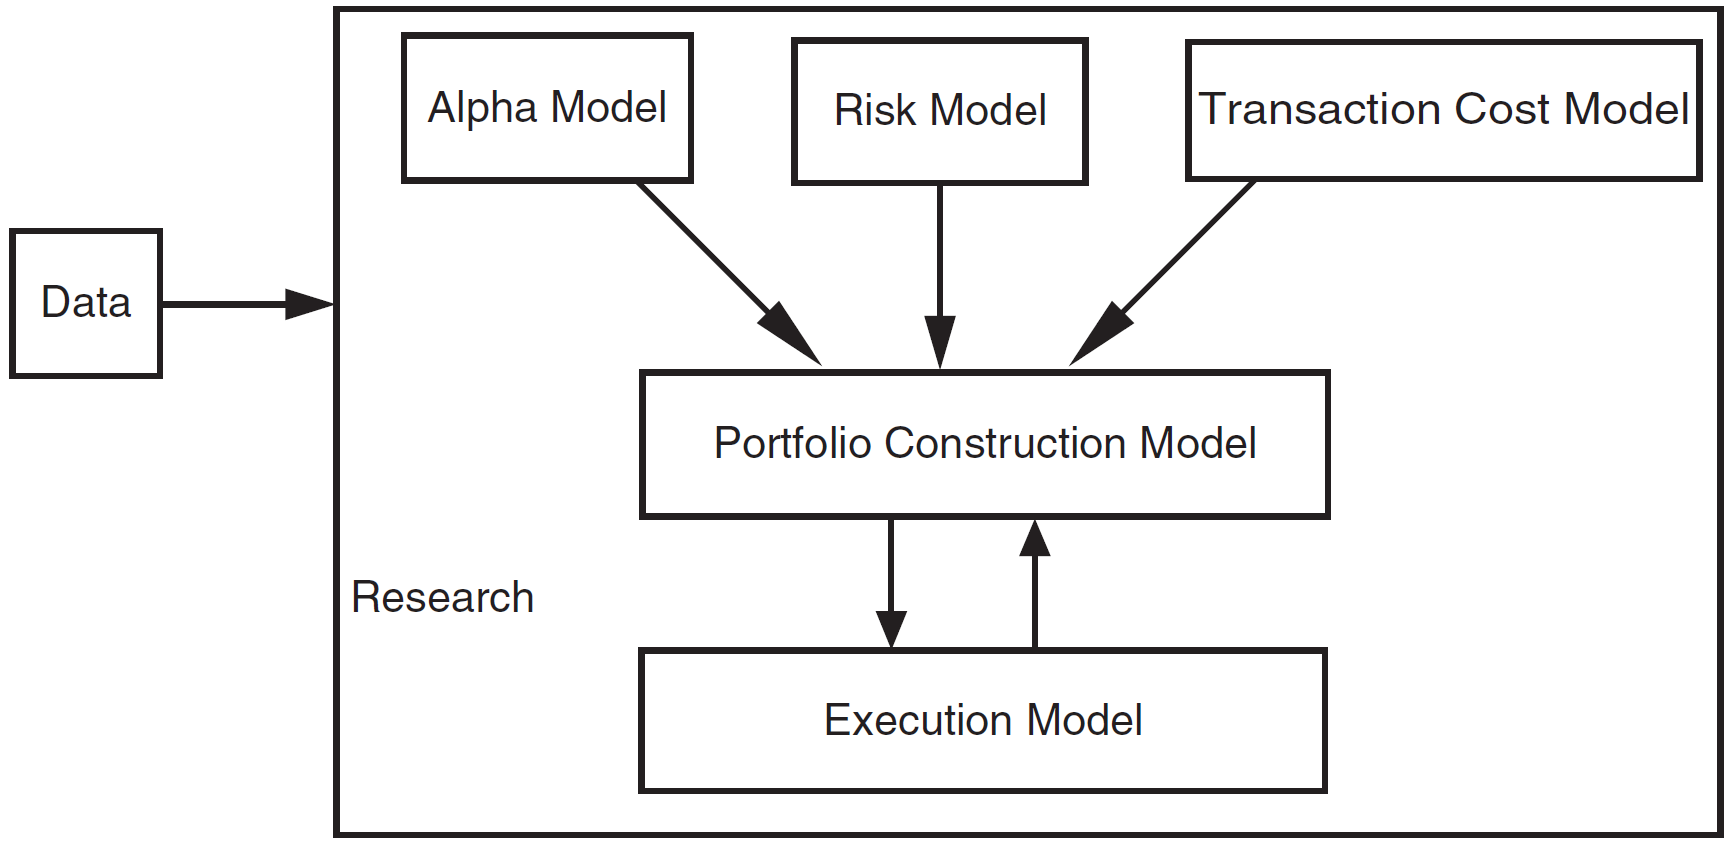
\includegraphics[width=.9\textwidth]{quantsys.png}
			\caption{Basic Structure of a Quant Trading Strategy}
			\label{fig:quantsys}
		\end{figure}

		The trading system has three modules -- an \textbf{alpha model}, a \textbf{risk model}, and a \textbf{transaction cost model} -- which feed into a \textbf{portfolio construction model}, which in turn interacts with the \textbf{execution model}. The \textit{alpha model} is designed to predict the future of the instruments the quant wants to consider trading for the purpose of generating returns. For example, in a trend-following strategy in the futures markets, the alpha model is designed to forecast the direction of whatever futures markets the quant has decided to include in his strategy.

		\textit{Risk models}, by contrast, are designed to help limit the amount of exposure the quant has to those factors that are unlikely to generate returns but could drive losses. For example, the trend follower could choose to limit his directional exposure to a given asset class, such as commodities, because of concerns that too many forecasts he follows could line up in the same direction, leading to excess risk; the risk model would contain the levels for these commodity exposure limits.

		\textit{The transaction cost model} is used to help determine the cost of whatever trades are needed to migrate from the current portfolio to whatever new portfolio is desirable to the portfolio construction model. Almost any trading transaction costs money, whether the trader expects to profit greatly or a little from the trade. Staying with the example of the trend follower, if a trend is expected to be small and last only a short while, the transaction cost model might indicate that the cost of entering and exiting the trade is greater than the expected profits from the trend.

		The alpha, risk, and transaction cost models then feed into a \textit{portfolio construction model}, which balances the tradeoffs presented by the pursuit of profits, the limiting of risk, and the costs associated with both, thereby determining the best portfolio to hold. Having made this determination, the system can compare the current portfolio to the new target portfolio, with the differences between the current portfolio and the target portfolio representing the trades that need to be executed.

		The current portfolio reflects the positions the quant trader currently owns. After running the portfolio construction model, the quant trader generates the new target portfolio weights. The difference between the two indicates the trades that now need to be executed, which is the job of the \textit{execution algorithm}. The execution algorithm takes the required trades and, using various other inputs such as the urgency with which the trades need to be executed and the dynamics of the liquidity in the markets, executes trades in an efficient and low-cost manner.

	\chapter{Alpha models}

		By conventional definition, alpha is the portion of the investor's return not due to the market benchmark, or, in other words, the value added (or lost) solely because of the manager. What is common to all pursuits of alpha is that they are in essence designed to time the selection and/or sizing of portfolio holdings.

		There are two types of alpha models: \textbf{theory-driven} and \textbf{data-driven}. Theory driven traders start with observations of the markets, think of a generalized theory that could explain the observed behavior, then rigorously test it with market data to see if the theory is shown to be either untrue or supported by the outcome of the test. Data-driven traders (``data miners'') believe that correctly performed empirical observation and analysis of the data can obviate the need for theory. They pursue to detect recognizable patterns in the data with careful application of the right techniques.

		\section{Theory-driven alpha models}

			\begin{figure}[htbp]
				\centering
				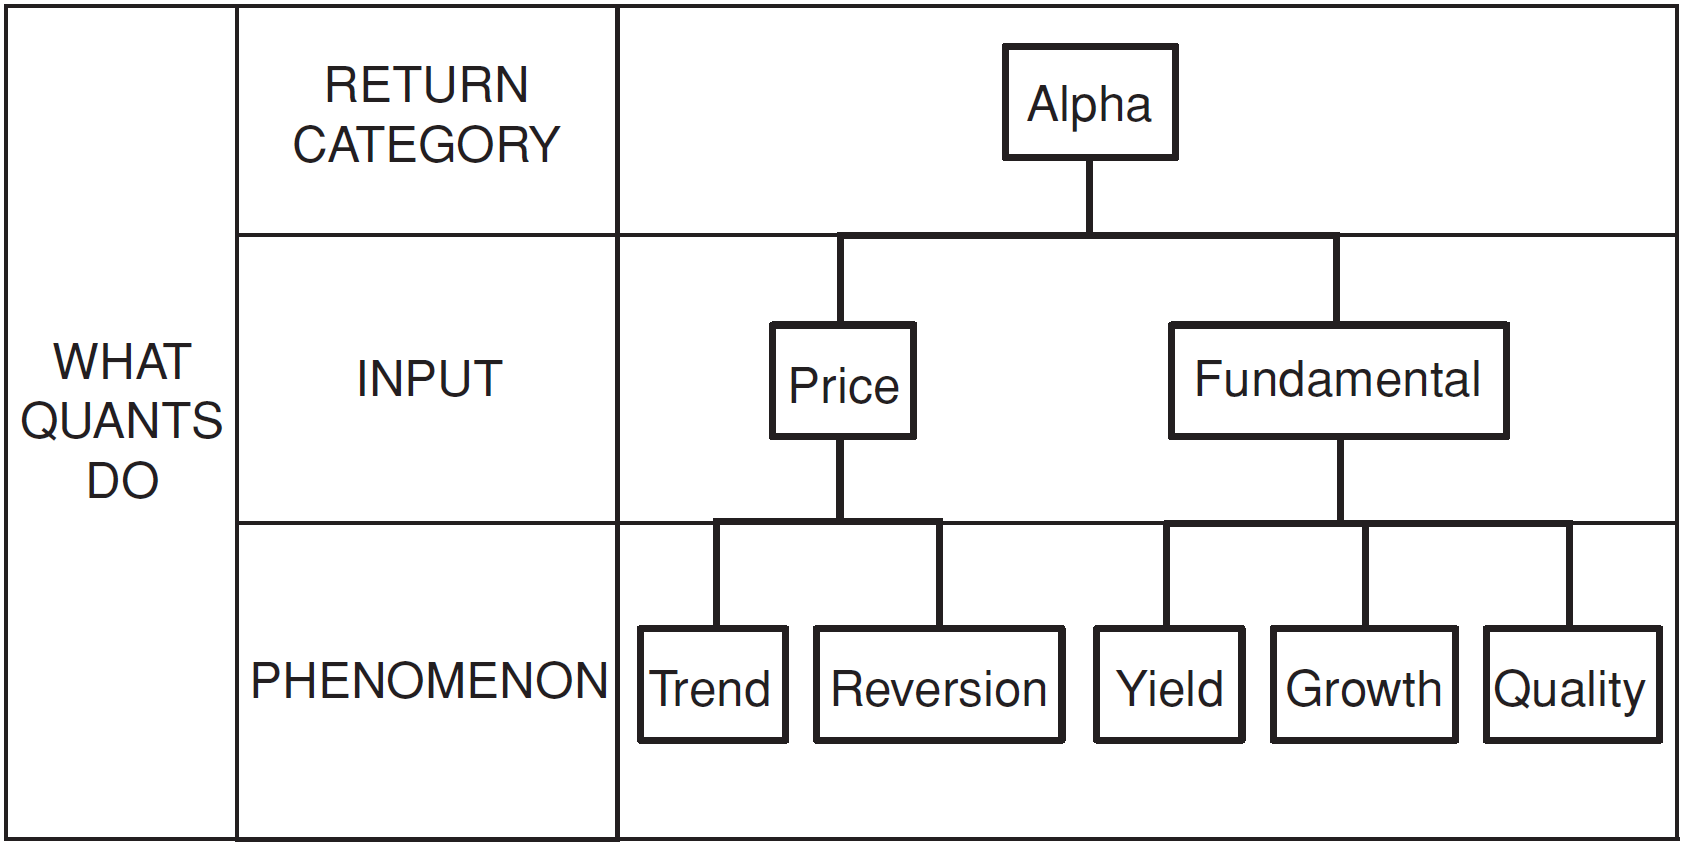
\includegraphics[width=.9\textwidth]{alphatheory.png}
				\caption{A taxonomy of theory-driven alpha models}
				\label{fig:alphatheory}
			\end{figure}

			Theory-driven alpha models can be classified as follows:
			\begin{itemize}
				\item Price-related data:
					\begin{itemize}
						\item trend;
						\item reversion.
					\end{itemize}
				\item Fundamental data:
					\begin{itemize}
						\item value/yield;
						\item growth;
						\item quality.
					\end{itemize}
			\end{itemize}

			\subsection{Strategies utilizing price-related data}

				\subsubsection{Trend following}

					Trend following is based on the theory that markets sometimes move for long enough in a given direction that one can identify this trend and ride it. The economic rationale for the existence of trends is based on the idea of consensus-building among market participants. It bears mentioning that there is an alternate explanation of why trends happen; it is affectionately known as the \textit{greater fools theory}. The idea here is that, because people believe in trends, they tend to start buying anything that's been going up and selling anything that's been going down, which itself perpetuates the trend. The key is always to sell your position to someone more ``foolish,'' and thereby to avoid being the last fool. Either theoretical explanation, coupled with the evidence in markets, seems a valid enough reason to believe in trends.

					Trend followers typically look for a significant move in a given direction in an instrument. They bet that, once a significant move has occurred, it will persist because this significant move is a likely sign of a growing consensus (or a parade of fools). There are many ways of defining what kind of move is significant, but the idea is the same regardless. Perhaps the most obvious and well-known example of a strategy that depends on trends is in the world of futures trading, or commodities trading advisors (CTAs). Figure~\ref{fig:MAtrend} illustrates the downward trend in equities that began in the fourth quarter of 2007. One way to define a trend for trading purposes, known as a moving average crossover indicator, is to compare the average price of the index over a shorter time period (e.g., 60 days) to that of a longer time period (e.g., 200 days). When the shorter-term average price is below the longer-term average price, the index is said to be in a negative trend, and when the shorter-term average price is above the longer-term average, the index is in a positive trend. As such, a trend follower using this kind of strategy might have gotten short the S\&P Index around the end of 2007, as indicated by the point at which the two moving averages cross over each other, and remained short for most or all of 2008.

					\begin{figure}[htbp]
						\centering
						\title{S\&P 500 Index, October 3, 2007 -- December 9, 2008}
						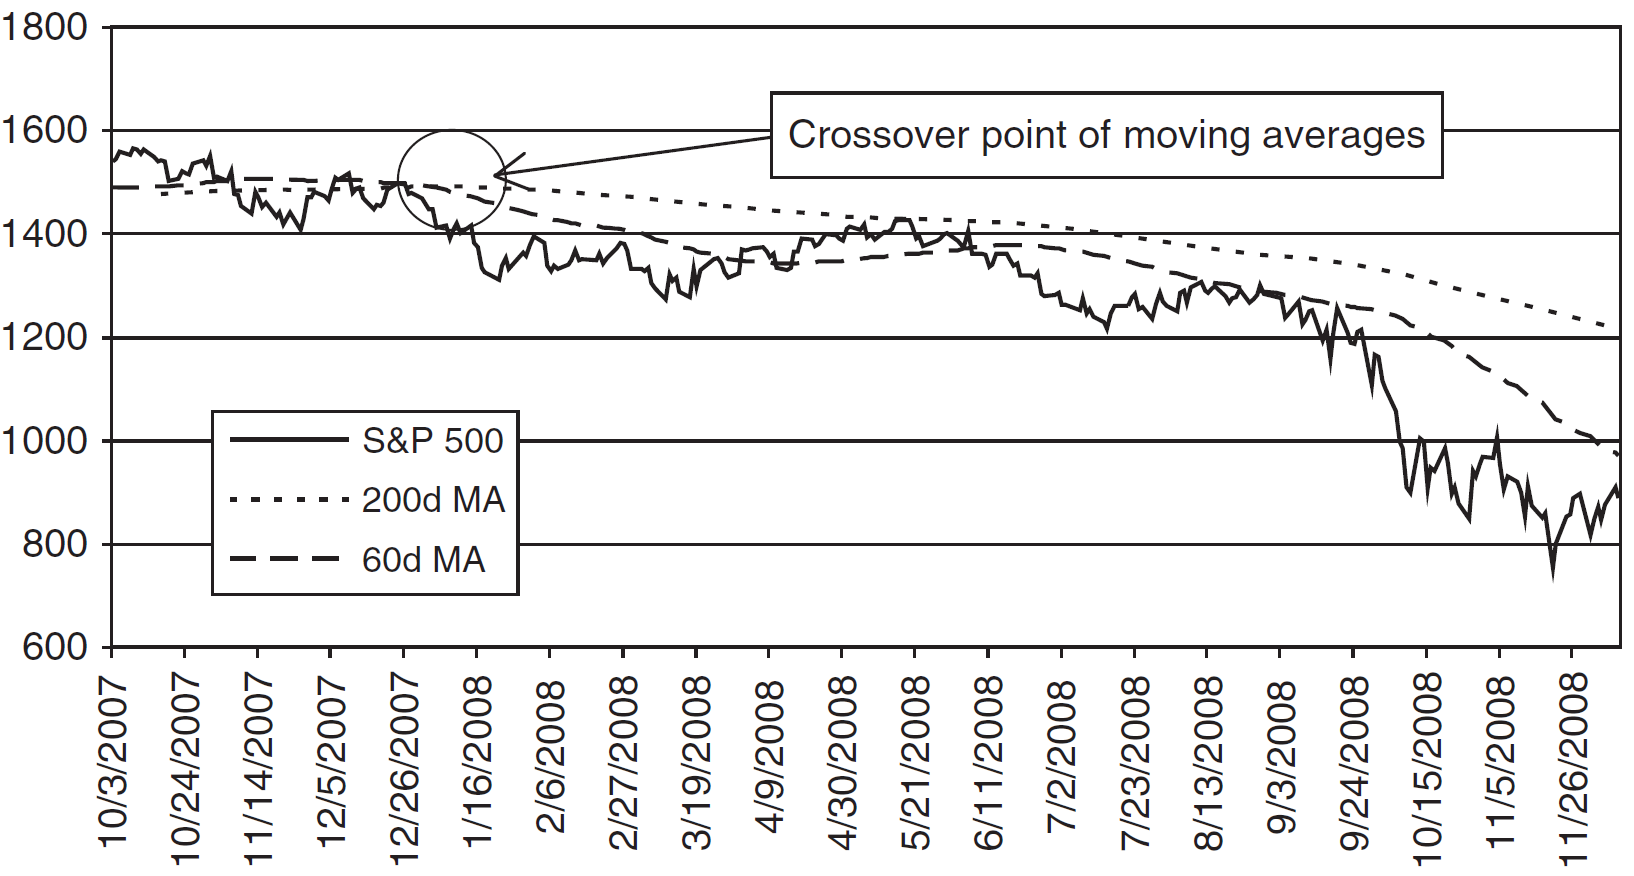
\includegraphics[width=.9\textwidth]{MAtrend.png}
						\caption{S\&P 500 Trend}
						\label{fig:MAtrend}
					\end{figure}

					Lest it seem like this is an overly rosy picture of trend following, it should be stated clearly: These strategies come with a great deal of risk alongside their lofty returns. The typical successful trend follower earns less than one point of return for every point of downside risk delivered. In other words, to earn 50 percent per year, the investor must be prepared to suffer a loss greater than 50 percent at some point. In short, the returns of this strategy are streaky and highly variable.

					This is not only true of trend following. Indeed, each of the major classes of alpha described in this chapter is subject to relatively long periods of poor returns. This is because the behaviors they seek to profit from in the markets are not ever-present but rather are unstable and episodic. The idea is to make enough money in the good times and manage the downside well enough in the bad times to make the whole exercise worthwhile.

				\subsubsection{Mean reversion}

					The theory behind mean reversion strategies is that there exists a center of gravity around which prices fluctuate, and it is possible to identify both this center of gravity and what fluctuation is sufficient to warrant making a trade. The rationale behind this theory can be found in a few ways. First, there are sometimes short-term imbalances among buyers and sellers due simply to liquidity that leads to an instrument being ``over-bought'' or ``oversold.'' To return to the example mentioned earlier, imagine that a stock has been added to a well-followed index, such as the S\&P 500. This forces any fund that is attempting to track the index to run out and buy the stock, and, in the short term, there might not be enough sellers at the old price to accommodate them. Therefore, the price moves up somewhat abruptly, which increases the probability that the price will reverse again at some point, when the excess demand from index buyers has subsided. Another rationale to explain the existence of mean-reverting behavior is that market participants are not all aware of each other's views and actions, and as they each place orders that drive a price toward its new equilibrium level, the price can overshoot due to excess supply or demand at any given time. Regardless of the cause of the short-term imbalance between supply and demand, mean reversion traders are frequently being paid to provide liquidity because they are bucking current trends and can therefore often buy on the bid and sell on the offer, thereby capturing the bid/ask spread.

					Interestingly, trend and mean reversion strategies are not necessarily at odds with each other. Longer-term trends can occur, even as smaller oscillations around these trends occur in the shorter term. In fact, some quants use both of these strategies in conjunction. Mean reversion traders must identify the current ``mean'' or ``equilibrium'' and then must determine what amount of divergence from that equilibrium is sufficient to warrant a trade. As in the case of trend following, there are a large number of ways of defining the ``mean'' and the reversal. It is worth noting that when discretionary traders implement mean reversion strategies, they are typically known as contrarians.

					Perhaps the best-known strategy based on the mean reversion concept is known as \textit{statistical arbitrage}, which bets on the convergence of the prices of similar stocks whose prices have diverged. Stat arb ushered in an important change in world view, one that focused on whether company A was over- or undervalued relative to company B rather than whether company A was simply cheap or expensive in itself. This important evolution would lead to the creation of many strategies based on forecasts of relative attractiveness.

					Figure~\ref{fig:reversionspread} shows a simplified example of the mean-reverting behavior evident between similar instruments, in this case Merrill Lynch (MER) and Charles Schwab (SCHW). The spread between these two companies oscillates rather consistently in a reasonably narrow range for long periods. This effect allows a trader to wait for significant divergences and then bet on a reversion back to the equilibrium level.

					\begin{figure}[htbp]
						\centering
						\title{SCHW vs. MER Daily Spread vs. Trailing Five-Day Spread, 2004 -- 2006}
						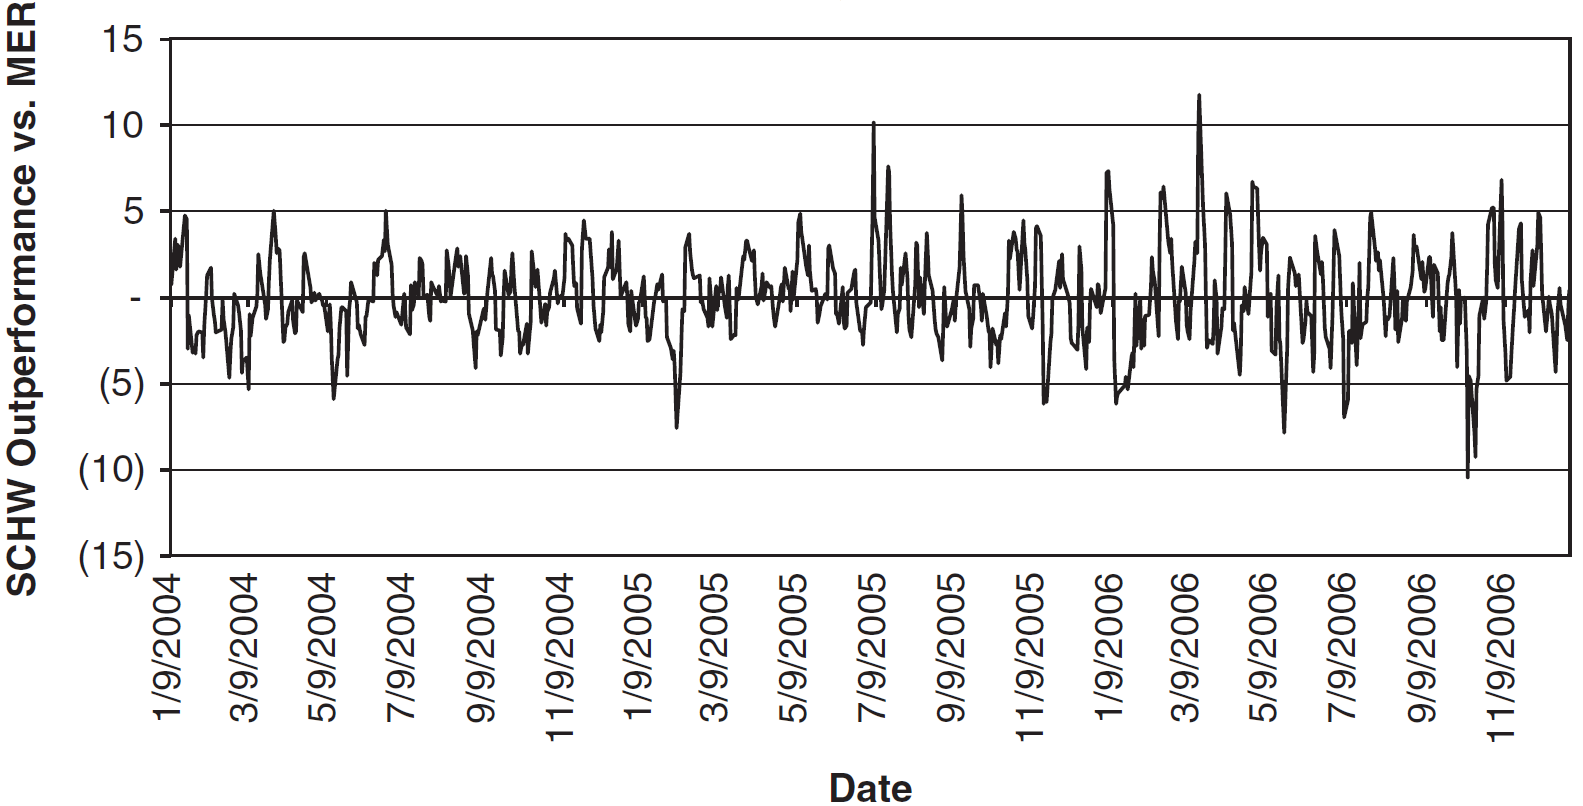
\includegraphics[width=.9\textwidth]{reversionspread.png}
						\caption{Mean Reversion Between SCHW and MER}
						\label{fig:reversionspread}
					\end{figure}

					Trend and mean reversion strategies represent a large portion of all quant trading. After all, price data are plentiful and always changing, presenting the quant with many opportunities to trade. It may be interesting to note that trend and mean reversion, though they are theoretically opposite ideas, both seem to work. How is this possible? Largely, it's possible because of different timeframes. It is obviously correct that both strategies can't possibly be made to be exactly opposite while both making money at the same time. However, there is no reason to create both strategies to be exactly the same. Trends tend to occur over longer time horizons, whereas reversions tend to happen over shorter-term time horizons. Figure~\ref{fig:snp500trendreversion} shows this effect in action. You can see that there are indeed longer-term trends and shorter-term mean reversions that take place. In fact, you can also see that the strategies are likely to work well at different times. From 2000 to 2002 and again in 2008, a trend strategy likely exhibits better performance, since the markets were trending very strongly during these periods. From 2003 to 2007, mean-reverting behavior was more prevalent. Yet both strategies are likely to have made money for the period as a whole.

					\begin{figure}[htbp]
						\centering
						\title {Trend and mean reversion in the  S\&P 500 Index}
						\begin{subfigure}[b] {0.9\textwidth}
							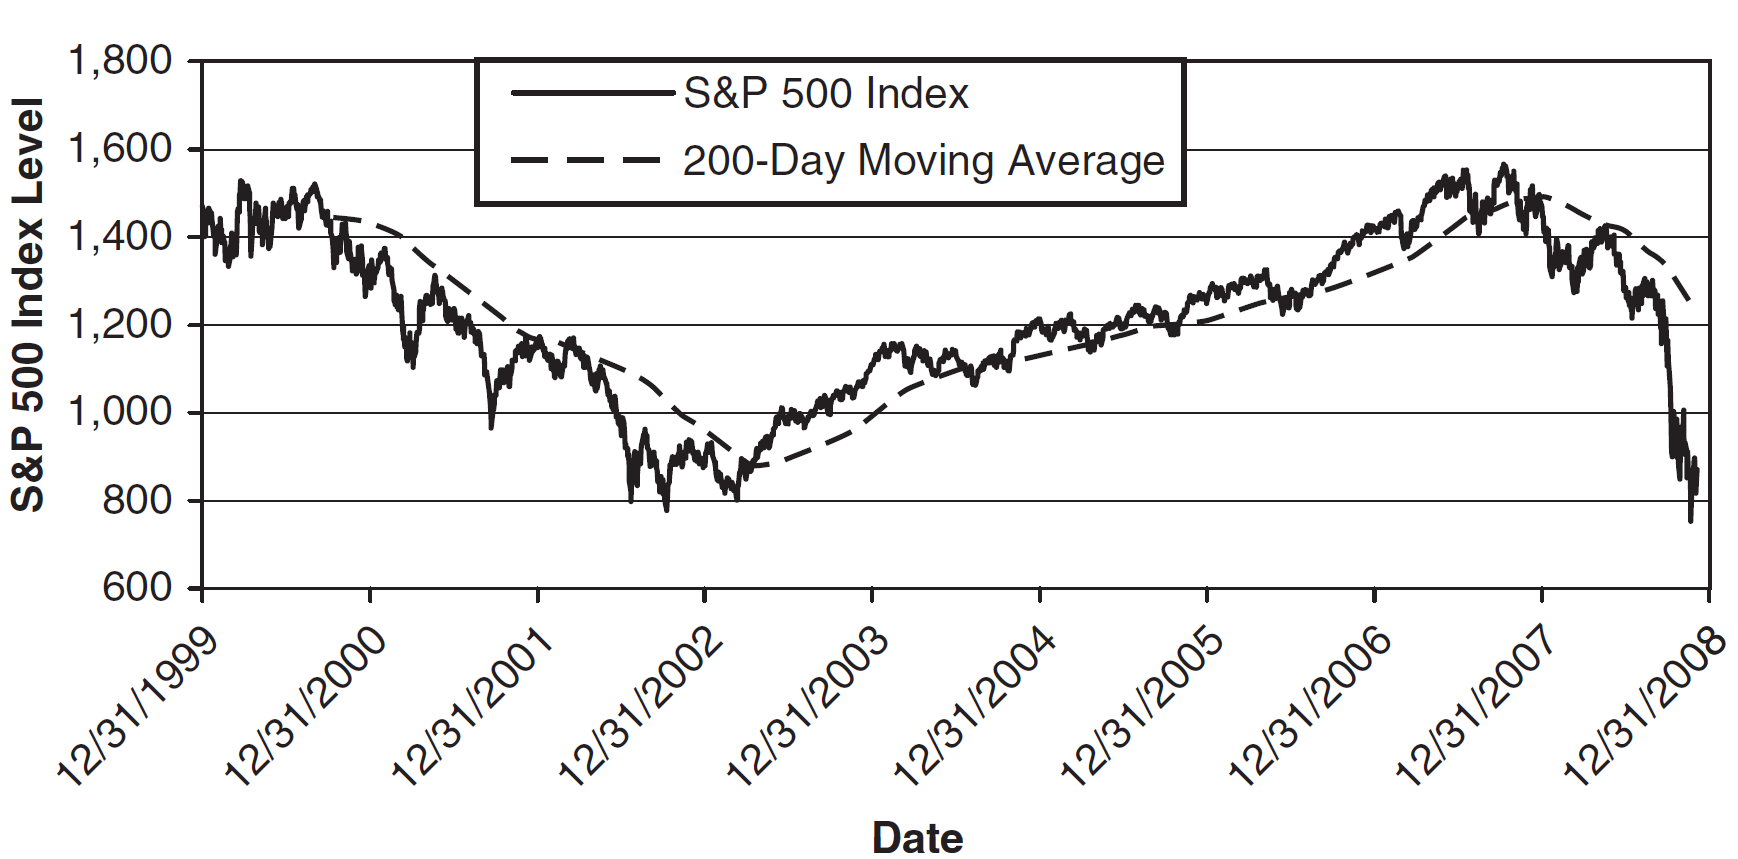
\includegraphics[width=\linewidth]{snp500trend.png}	
						\end{subfigure}
						\begin{subfigure}[b] {0.9\textwidth}
							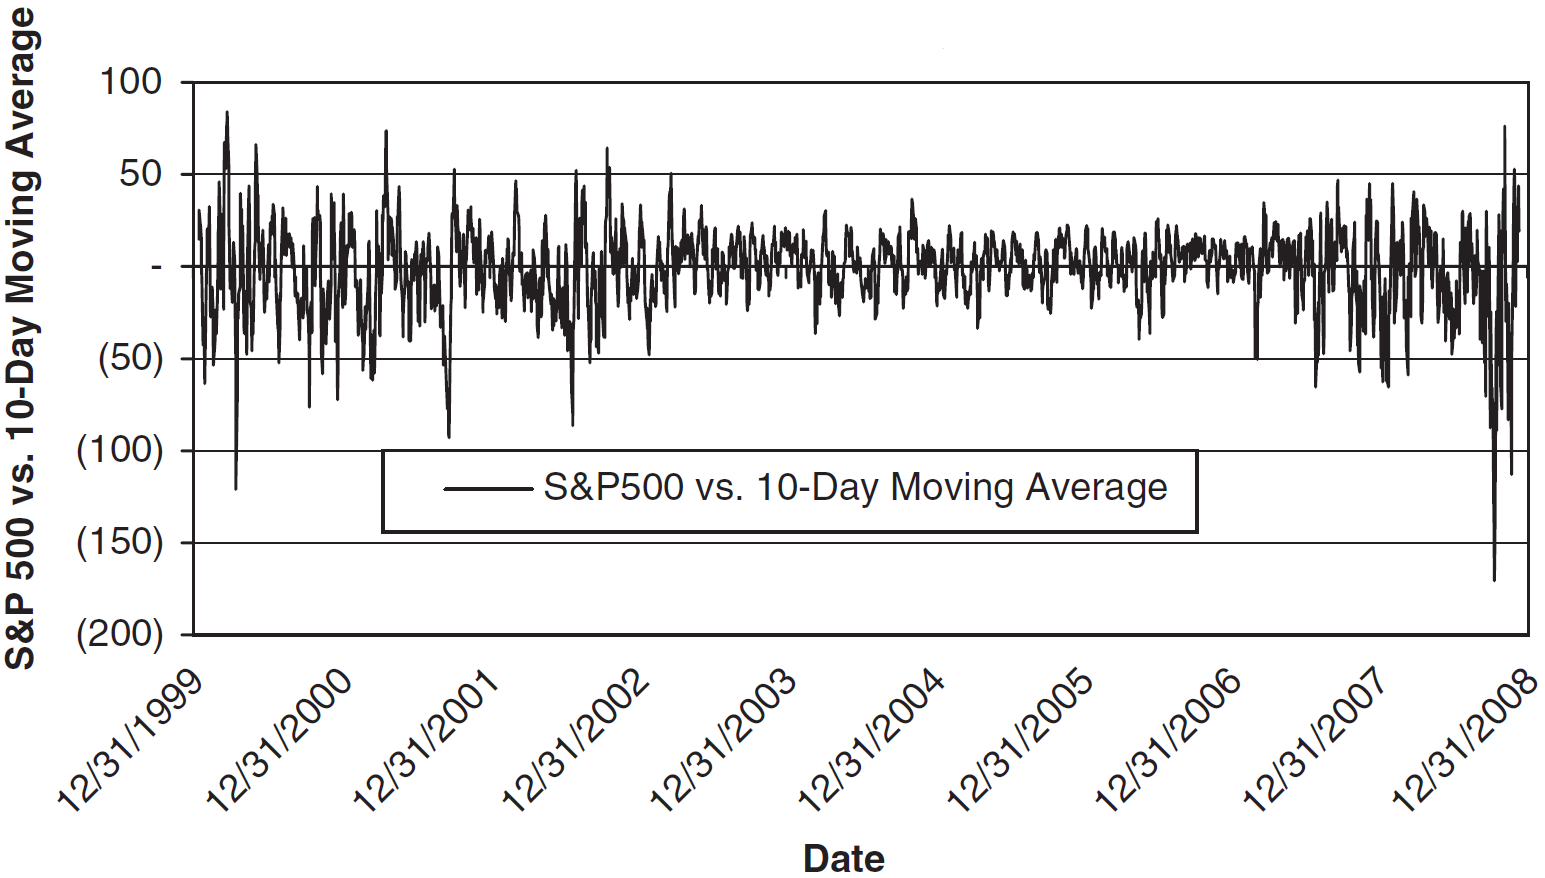
\includegraphics[width=\linewidth]{snp500reversion.png}	
						\end{subfigure}
						\caption{Trend and reversion coexisting}
						\label{fig:snp500trendreversion}
					\end{figure}

			\subsection{Strategies utilizing fundamental data}

				\subsubsection{Value/yield}

					Value strategies are well known and are usually associated with equity trading, though such strategies can be used in other markets as well. There are many metrics that people use to describe value in various asset classes, but most of them end up being ratios of some fundamental factor versus the price of the instrument, such as the \textbf{price-to-earnings (P/E) ratio}. Quants tend to invert such ratios, keeping prices in the denominator. An inverted P/E ratio, or an E/P ratio, is also known as \textit{earnings yield}. Note that investors traditionally already do this with dividends, hence the \textit{dividend yield}, another commonly used measure of value. The basic concept of value strategies is that the higher the yield, the cheaper the instrument. The benefit of the conversion of ratios to yields is that it allows for much easier and more consistent analysis. Because ratios with price in the numerator and some fundamental figure in the denominator exhibit of this sort of misbehavior, quants tend to use the inverted yield forms of these same ratios. This idea is demonstrated in Figure~\ref{fig:PEratio}, which shows that the E/P ratio is well behaved for any level of earnings per share for a hypothetical stock with a price greater than \$1 (in the example, we used \$20 per share as the stock price). By contrast, the P/E ratio is rather poorly behaved and does not lend itself well to analysis and is not even properly defined when earnings per share are zero.

					\begin{figure}[htbp]
						\centering
						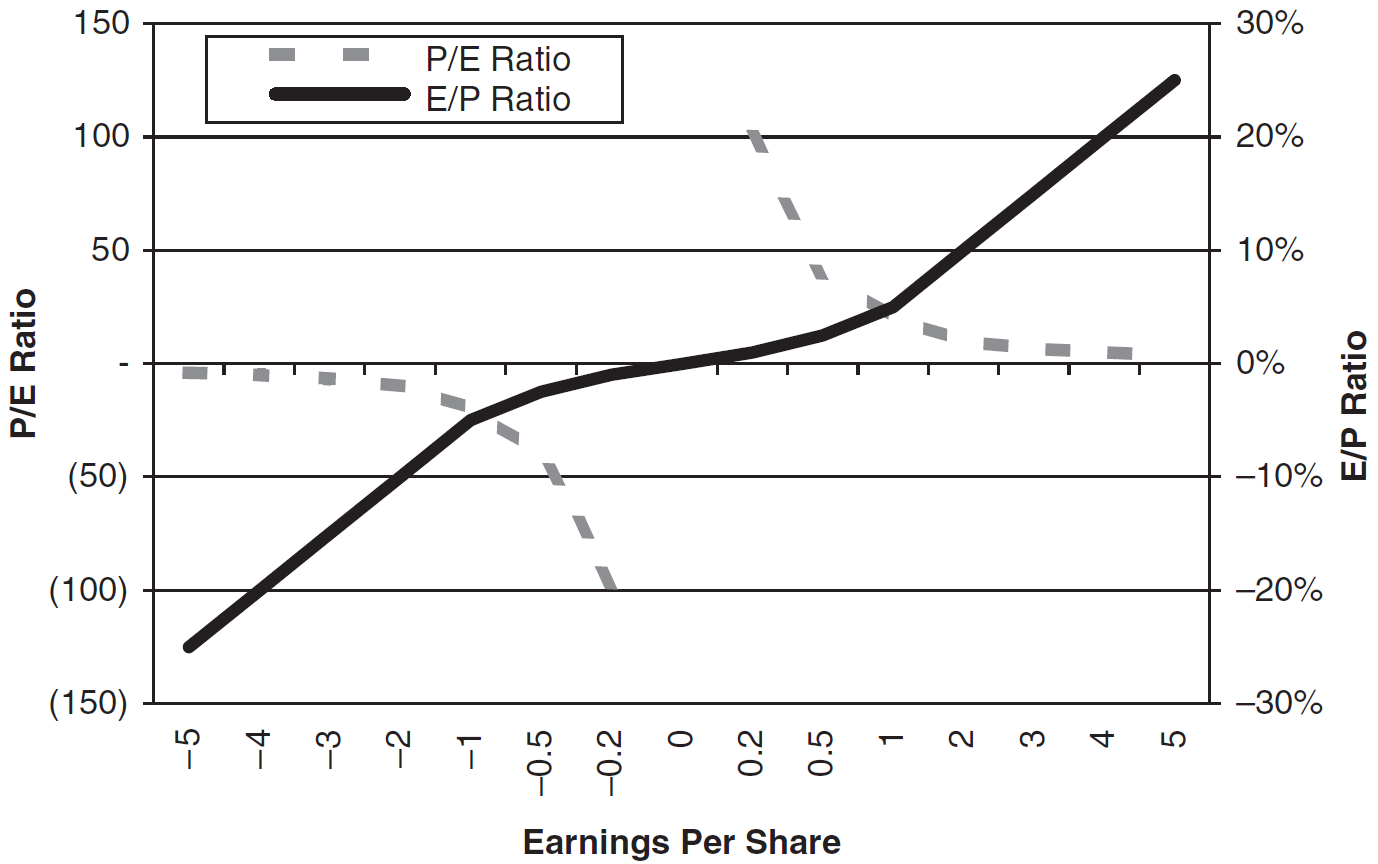
\includegraphics[width=.9\textwidth]{PEratio.png}
						\caption{P/E versus E/P (``Earnings Yield'')}
						\label{fig:PEratio}
					\end{figure}

					Most often, value is thought of as a strategy that is defined by ``buying cheap.'' In reality, the idea behind value investing is that markets tend to overestimate the risk in risky instruments and possibly to underestimate the risk in less risky ones. Therefore, it can pay off to own the more risky asset and/or sell the less risky asset. The argument for this theory is that sometimes instruments have a higher yield than is justified by their fundamentals simply because the market is requiring a high yield for that kind of instrument at the moment. An investor who can purchase this instrument while it has a high yield can profit from the movement over time to a more efficient, ``fair'' price.\footnote{Ray Ball, a professor of accounting at the University of Chicago's Booth School of Business, wrote a paper, ``Anomalies in Relationships Between Securities' Yields and Yield-Surrogates'', which echoes the idea that higher-yielding stocks—those with higher earnings yields—are likely those for which investors expect to receive higher returns and greater risks.}

					When done on a relative basis, that is, buying the undervalued security and selling the overvalued one against it, this strategy is also known as a \textit{carry trade}. One receives a higher yield from the long position and finances this with the short position, on which a lower yield must be paid. The spread between the yield received and the yield paid is the carry. For instance, one could sell short \$1,000,000 of U.S. bonds and use the proceeds to buy \$1,000,000 of higher-yielding Mexican bonds. Graham and Dodd, in their landmark book ``Security Analysis'', propose that value trading offers investors a margin of safety. In many respects, this margin of safety can be seen clearly in the concept of carry. If nothing else happens, a carry trade offers an investor a baseline rate of return, which acts as the margin of safety Graham and Dodd were talking about.

					Carry trading is an enormously popular kind of strategy for quants (and discretionary traders) in currencies, where the currency of a country with higher short-term yields is purchased against a short position in the currency of a country with relatively low short-term yields. For example, if the European Central Bank's target interest rate is set at 4.25 percent, whereas the U.S. Federal Reserve has set the Fed Funds rate at 2 percent, a carry trade would be to buy Euros against the U.S. dollar. This is a classic value trade because the net yield is 2.25 percent (4.25 percent gained on the Euro position, less 2 percent paid in U.S. interest), and this provides a margin of safety. If the trade doesn't work, the first 2.25 percent of the loss on it is eliminated by the positive carry.

					Another important example of value trading is in equities, where many kinds of traders seek to define metrics of ``cheapness,'' such as \textbf{earnings before interest, taxes, depreciation, and amortization (EBITDA) versus enterprise value (EV)} or \textbf{book value to price}. Book value per share versus price (\textbf{book yield} or \textbf{book-to-price}) is also a fairly common factor, as it has been among quants since Fama and French popularized it in their papers. Most quant equity traders who use value strategies are seeking relative value rather than simply making an assessment of whether a given stock is cheap or expensive. This strategy is commonly known as quant long/short (QLS). QLS traders tend to rank stocks according to their attractiveness based on various factors, such as value, and then buy the higher-ranked stocks while selling short the lower-ranked ones. The presumption is that a stock with a higher book-to-price ratio might outperform stocks with lower book-to-price ratios over the coming quarters.

				\subsubsection{Growth}

					Growth strategies seek to make predictions based on the asset in question's expected or historically observed level of economic growth. Some examples of such ideas could be \textbf{gross domestic product (GDP) growth} or \textbf{earnings growth}. That a given stock is a growth asset implies nothing about its valuation or yield. The theory here is that, all else equal, it is better to buy assets that are experiencing rapid economic growth and/or to sell assets that are experiencing slow or negative growth. Some growth metrics, like the \textbf{price/earnings-to-growth (PEG) ratio} (PE ratio vs. EPS growth rate), are basically a forward-looking concept of value, that is, they compare growth expectations to value expectations to see whether a given instrument is fairly pricing in the positive or negative growth that the trader believes the asset will likely experience. If you expect an asset to grow rapidly but the market has already priced the asset to account for that growth, there is no growth trade to be made. In fact, if the market has priced in a great deal more growth than you expect, it might even be reasonable to short the instrument. But certainly many forms of growth trading are simply focused on buying rapidly growing assets regardless of price and selling assets with stagnant or negative growth, even if they are very cheap (or offer high yields) already.

					The justification for growth investing is that growth is typically experienced in a trending manner, and the strongest growers are typically becoming more dominant relative to their competitors. In the case of a company, you could see the case being made that a strong grower is quite likely to be in the process of winning market share from its weaker-growing competitors. Growth investors try to be early in the process of identifying growth and, hence, early in capturing the implied increase in the future stature of a company. We can see examples of both macroeconomic growth strategies and microeconomic growth strategies in the quant trading world. At the macro level, some foreign exchange trading concepts are predicated on the idea that it is good to be long currencies of countries that are experiencing relatively strong growth, because it is likely that these will have higher relative interest rates in the future than weaker-growth or recession economies, which makes this a sort of forward-looking carry trade.

					In the quant equity world, the QLS community frequently also utilizes signals relating to growth to help diversify their alpha models. Note that an important variant of growth trading utilized by a wide variety of quant and discretionary equity traders focuses on analysts' earnings estimate revisions. Sell-side analysts working at various brokerage houses publish their estimates and release occasional reports about the companies they cover. The thesis is identical to any other growth strategy, but the idea is to try to get an early glimpse of a company's growth by using the analysts' expectations rather than simply waiting for the company itself to report its official earnings results. Because this strategy depends on the views of market analysts or economists, it is called a \textit{sentiment-based strategy} (as opposed to \textit{fundamental strategies} that use official releases by corporations or governments). The quant community does not universally agree that sentiment-based strategies, such as the estimate revision idea just mentioned, are nothing more than variants of growth strategies, but it is my experience that these two are highly enough correlated in practice to warrant their being treated as close cousins. After all, too often Wall Street analysts' future estimates of growth look a lot like extrapolations of recent historical growth.

				\subsubsection{Quality}

					The final kind of theory-driven fundamental alpha is called \textit{quality}. A quality investor believes that, all else being equal, it is better to own instruments that are of high quality and better to sell or be short instruments of poor quality. The justification for this strategy is that capital safety is important, and neither growth nor value strategies really capture this concept. A strategy focused on owning higher-quality instruments may help protect an investor, particularly in a stressful market environment. Not coincidentally, these are frequently termed \textit{flight-to-quality} environments. This kind of strategy is easily found in quant equity trading but not as commonly in macroeconomic types of quant trading. A typical kind of QLS signal focused on quality might look at the debt-to-equity ratios of stocks to help determine which ones to buy, the idea being that less-leveraged companies are considered higher quality than more-leveraged companies, all else equal. Another example is an \textit{earnings quality} signal, which attempts to measure how close are a company's true economic earnings (as measured by, say, the free cash flow) to the reported earnings-per-share numbers. Such strategies especially gained prominence in the wake of the accounting scandals of 2001 and 2002 (Enron and WorldCom, for example), which highlighted that sometimes publicly traded companies are run by folks who are trying harder manage their financial statements than manage their companies. Some quality signals focus on the diversification of a company's sources of earnings (or of the drivers of GDP growth for an economy), with the idea being that higher-quality companies will have more diversified earnings sources. Recently, quality has been a particularly important issue, and a particularly successful factor, in predicting the relative prices of banking stocks, probably because of the credit crisis-roiled markets in 2008. In particular, some quality factors helped traders detect, avoid, and/or sell short those banks with the most leverage or the most exposure to mortgage-related businesses, thereby allowing these traders to avoid or even profit from the 2008 credit crisis.

		\section{Data-driven alpha models}

			Data mining, when done well, is based on the premise that the data tell you what is likely to happen next, based on some patterns that are recognizable using certain analytical techniques. When used as alpha models, the inputs are usually sourced from exchanges (mostly prices), and these strategies typically seek to identify patterns that have some explanatory power about the future.

			There are two advantages to these approaches. First, compared with theory-driven strategies, data mining is considerably more technically challenging and far less widely practiced. This means that there are fewer competitors, which is helpful. Second, data-driven strategies are able to discern behaviors whether they have been already named under the banner of some theory or not, which allows them to discover that something happens without having to understand why.
 			
 			For example, many high-frequency traders favor an entirely empirical, data-mining approach when designing their short-term trading strategies for equity, futures and foreign exchange markets. These data-mining strategies may be more successful in high frequency because, if designed well, they are able to discern how the market behaves without having to worry about the economic theory or rationalization behind this behavior. Since there is not much good literature at this time about the theoretical underpinnings of human and computerized trading behaviors at very short-term time horizons (i.e., minutes or less), an empirical approach may actually be able to outperform a theoretical approach at this timescale. Furthermore, at this timescale there is so much more data to work with that the empirical researcher has a better chance of finding statistically significant results in his testing.

			However, data-mining strategies also have many shortcomings. The researcher must decide what data to feed the model. If he allows the model to use data that have little or no connection to what he is trying to forecast he may find results that are seemingly significant but are in reality entirely spurious. Furthermore, if the researcher chooses the set of all data generally thought to be useful in predicting markets, the amount of searching the algorithms must conduct is so enormous as to be entirely impractical. To run a relatively thorough searching algorithm over, say, two years of intraday tick data, with a handful of inputs, might take a single computer processor about three months of continuous processing before it finds the combinations of data that have predictive power. If this was not difficult enough, whatever strategies are found in this manner require the past to look at least reasonably like the future, although the future doesn't tend to cooperate with this plan very often or for very long. To adjust for this problem, the data-mining strategy requires nearly constant adjustment to keep up with the changes going on in markets, an activity that has many risks in itself.
			
			A second problem is that generating alphas using solely data-mining algorithms is a somewhat dubious exercise. The inputs are noisy, containing a great number of false signals that act like traps for data miners. In general, strategies that use data-mining techniques to forecast markets do not work, though there are a few exceptions. It is worth noting that the strategies employed by most successful data miners end up looking a lot like trending or reverting strategies.

		\section{Implementing strategies}

			\subsection{Forecast target}

				The first key component of implementation is to understand exactly what the model is trying to forecast. Models can forecast the direction, magnitude, and/or duration of a move and furthermore can include an assignment of confidence or probability for their forecasts. Many models forecast direction only, most notably the majority of trend-following strategies in futures markets. They seek to predict whether an asset price will rise or fall, and nothing more. Still others have specific forecasts of the size of a move, either in the form of an expected return or a price target. Some models, though they are far less common, also seek to identify how long a move might take. If the forecasted behavior is not exhibited within the defined time window, the trade is considered a failure and is exited.

				Finally, the \textit{signal strength} is an important (but not ubiquitous) aspect of the quant model. Signal strength is defined by a larger expected return and/or by a higher likelihood of a return. The larger the expected return (i.e., the further the price target is from the current price), the greater the strength of the signal, holding confidence levels constant. Similarly, the more confidence in a signal, the greater the signal strength, holding expected returns constant. In general, though certainly not always, a higher level of signal strength results in a bigger bet being taken on a position.


			\subsection{Time horizon}

				The next key component to understanding implementation of the alpha model is time horizon. Some quant models try to forecast literally microseconds into the future; others attempt to predict behavior a year or more ahead. Most quant strategies have forecast horizons that fall in the range of a few days to several months. Notably, a strategy applied to the very short term can look quite different than it would if the exact same idea was applied to the very long term. The same strategy, applied over different time horizons, can produce markedly different -- even opposite -- positions.

				A classification may be helpful in understanding the distinctions among quant trading strategies by time horizon. \textit{High-frequency} strategies are the fastest, making forecasts that go no further than the end of the current trading day. \textit{Short-term} strategies, the second category, tend to hold positions from one day to two weeks. \textit{Medium-term} strategies make forecasts anywhere from a few weeks to a few months ahead. Finally, \textit{long-term} strategies hold positions for several months or longer.

			\subsection{Bet structure}

				The next key component of an alpha model is bet structure, which, in turn, is based on how the alpha model generates its forecast. Models can be made to forecast either an instrument in itself or an instrument \textit{relative} to others. For example, a model could forecast that gold is cheap and its price is likely to rise or that gold is cheap relative to silver, and that gold is therefore likely to outperform silver. When looking at relative forecasts, one can forecast the behavior of smaller clusters (e.g., pairs) or larger clusters (e.g., sectors). Smaller clusters have the advantage of being easier to understand and analyze. In particular, pairs are primarily attractive because, in theory, one can carefully select instruments that are directly comparable.

				However, pairs have several comparative disadvantages. Very few assets can actually be compared so precisely and directly with one other instrument, rendering a major benefit of pairs trading impracticable. Two Internet companies might each depend significantly on revenues from their respective search engines, but they may differ along other lines. One could have more of a content-driven business while the other uses advertising to supplement the search engine revenues.Meanwhile, one could find other companies with strong advertising or content businesses, each of which shares some characteristics and sector-effects with the first pair. Here the trader is presented with a dilemma: which pairs are actually the best to use? Or to put it another way, how should the trader's pairs best be structured?

				Another approach is to make bets based on larger clusters or groups. Researchers group securities together primarily in an effort to isolate and eliminate common effects among the group. A large part of the point of grouping stocks within their market sector, for example, is to eliminate the impact of a general movement of the sector and thereby focus on the \textit{relative} movement of stocks \textit{within} the sector. It turns out to be extremely difficult to isolate group effects with a group size of merely two. On the other hand, larger clusters allow for a cleaner distinction between group behavior and idiosyncratic behavior, which is beneficial for many quant strategies. As a result, most quants who trade in groups tend to use larger groups than simply pairs when they make relative bets.

				Researchers also must choose \textit{how} they create these clusters, either using statistical techniques or using heuristics (e.g., fundamentally defined industry groups). There are many statistical techniques aimed at discerning when things are similar to each other or when they belong together as a group. However, statistical models can be fooled by the data, leading to bad groupings. For example, there may be periods during which the prices of Internet stocks behave like the price of corn. This may cause the statistical model to group them together, but Internet stocks and corn are ultimately more different than they are similar, and most fundamental grouping approaches would never put them together. Furthermore, any time that the market regime changes, the relationships among instruments frequently also change, which can lead the system to mistakenly group things together that no longer will behave like each other.

				Alternatively, groups can be defined heuristically. Asset classes, sectors, and industries are common examples of heuristically defined groups. They have the advantage of making sense and being defensible theoretically, but they are also imprecise and possibly too rigid. Rigidity in particular can be a problem because over time, similarities among instruments change. Sometimes stocks and bonds move in opposite directions, and sometimes they move in the same direction. Because the correlation between these two asset classes moves in phases, it can be very tricky to analyze the relationship theoretically and make a static, unchanging declaration that they belong in the same group or in different groups. As a result, most grouping techniques (and by extension, most strategies that are based on relative forecasts), whether statistically driven or human-made, suffer from changes in market regime that cause drastic changes in the relationships among instruments.

				In evaluating alpha-oriented strategies, this distinction among bet structures, most notably between intrinsic (single security) bets versus relative (multi-security) bets, is rather important. The behavior of a given type of alpha model is very different if it is implemented on an instrument by itself than it would be if implemented on a group of instruments relative to each other. It is critical to balance the risks and benefits of the various approaches to grouping. In general, relative alpha strategies tend to exhibit smoother returns during normal times than intrinsic alpha strategies, but they can also experience unique problems related to incorrect groupings during stressful periods. Some quants attempt to mitigate the problems associated with any particular grouping technique by utilizing several grouping techniques in concert. For example, one could first group stocks by their sectors but then refine these groupings using a more dynamic statistical approach that reflects recent correlations among the stocks.

				Also, it is worth clarifying one piece of particularly unhelpful, but widely used, hedge fund industry jargon: \textit{relative value}. This term refers to strategies that utilize a relative bet structure, but the \textit{value} part of the term is actually not useful. Certainly strategies that make forecasts based on a notion of the relative valuation of instruments are quite common. However, most strategies called relative value have little to do with value investing. Relative mean reversion strategies, relative momentum strategies, and other kinds of relative fundamental strategies are all commonly referred to as relative value.

			\subsection{Investment universe}

				A given strategy can be implemented in a variety of instruments, and the quant must choose which ones to include or exclude. The first significant choice a quant makes about the investment universe is \textit{geography}. A shortterm relative mean reversion strategy traded on stocks in the United States might not behave similarly to the same strategy applied to stocks in Hong Kong. The researcher must decide where to apply the strategy. The second significant choice a quant makes about the investment universe relates to its \textit{asset class}. A growth strategy applied to foreign exchange markets might behave differently than one applied to equity indices. The quant must decide what asset classes to trade with each strategy. A third significant choice a quant must make about the investment universe relates to the \textit{{instrument class}}. Equity indices, as accessed through the futures markets, behave differently than single stocks, even though both belong to the equity asset class. Also, the liquidity characteristics and nature of the other participants in a given market differ from one instrument class to another, and these are some of the considerations quants must make regarding what kinds of instruments to trade. Finally, in some cases, quants may include or exclude specific groups of instruments for a variety of reasons.

				The choice of an investment universe is dependent on several strong preferences that quants tend to have. First, the quant generally prefers liquidity in the underlying instruments so that estimations of transactions costs are reliable. Second, quants generally require large quantities of high-quality data. In general, such data can be found in highly liquid and developed markets. Third, quants tend to prefer instruments that behave in a manner conducive to being predicted by systematic models. Returning to the example of biotechnology stocks, some quants exclude them because they are subject to sudden, violent price changes based on events such as government approval or rejection of their latest drug. Although physician with a biotech specialization may have some intuitions on this subject, it’s simply not something that most quants can model. As a result of these preferences, the most typical asset classes and instruments in which one can find quants participating are common stocks, futures (especially on bonds and equity indices), and foreign exchange markets. Some strategies might trade the fixed income asset class using instruments other than futures (e.g., swaps or cash bonds), though these are significantly less common today than they were in the middle or late 1990s. Geographically, the bulk of quant trading occurs in the United States, developed Europe, and Japan, with lesser amounts done in other parts of North America and developed Asia. Quants are almost completely absent from illiquid instruments, or those traded ``over the counter'' (OTC), such as corporate or convertible bonds, and are rarely found in emerging markets.

				This last fact may change going forward as OTC markets become better regulated and electronic. But that also implies that the liquidity of these markets will improve. As such, this notion of liquidity is perhaps the simplest way to summarize in one dimension the salient characteristics of the trading universe for a strategy. After all, more liquid instruments also tend to offer more high-quality data and to be more conducive to being forecast, on average.

			\subsection{Model specification}

				Any differences in the way a quant chooses to specify or define an idea for her strategy might lead it to behave quite differently than other choices would have. For example, there could be multiple ways to define a trend. Some simply compute the total return of an instrument over some historical period, and if that number is positive, a positive trend is identified (a negative return would constitute a negative trend). Other trend traders use moving average approaches to look for prices to rise above or below recent average prices and so determine the presence of a trend. Still other trend strategies seek to identify the breakout of the very early stages of a trend, found using specific price patterns they believe are present in this critical phase, but they do not attempt to determine whether a long-term trend is actually in place or not.

				The specification of the details of a model is also an area in which some quants utilize machine learning or data-mining techniques. Fitting models to the data and setting parameter values is a problem to which machine learning techniques are better suited and more widely used. In essence, machine learning techniques are applied to determine the optimal set of specifications for a quant model. Machine learning algorithms are designed to provide an intelligent and scientifically valid way of testing many potential sets of specifications without overfitting.

				A subset of the problem of specifying a model relates to how often the models themselves are adjusted for more recent data. This process is known as refitting because some of the same work that goes on in the original research process is repeated in live trading in an attempt to refresh the model and make it as adaptive as possible to current market conditions. Because this can be a computationally intensive process, sometimes involving millions or even billions of calculations, many quants refit their models infrequently or not at all. Refitting also leads to a greater risk of overfitting, a very treacherous problem indeed, since spurious and fleeting relationships may be mistaken for valid, lasting ones.

			\subsection{Run frequency}

				A final component of building a given alpha model is determining the run frequency, or the frequency with which the model is actually run to seek new trading ideas. Some quants run their models relatively infrequently—for example, once per month. At the other extreme, some run their models more or less continuously, in real time. There is an interesting tradeoff that quants must manage here. Specifically, increasing the frequency of model runs usually leads to a greater number of transactions, which means more commissions paid to brokers and higher transaction costs. Also, more frequent model runs lead to a greater probability that the model is moving the portfolio around based on noisy data that doesn't actually mean that much. This, in turn, would mean that the increased transaction costs would cause little or no incremental improvement in the alpha generated by the strategy and would thereby reduce its overall profitability.

				On the other hand, less frequent model runs lead to a smaller number of larger-sized trades. These are expensive in a different way, namely in terms of the impact these trades can have on the marketplace. If models are run too infrequently, then at those times when they are run they could want to make very significant changes to the currently held portfolio. This would mean transacting larger blocks of trades, which would likely cost more in terms of ``moving the market.'' Less frequent model runs are also prone to problems associated with the moment of observation of markets. If a strategy is run once a month, it could miss opportunities to trade at more favorable prices that occur during the month while the model is dormant. Alternatively, the model may attempt in vain to trade at attractive, but quickly fleeting, prices that occur if there has been some aberration just around the time of the model being run. Whether more frequent or less frequent model runs are better depends on many other aspects of the strategy, most especially the time horizon of the forecast and the kinds of inputs. In the end, most quants run their models no less than once a week, and many run continuously throughout the day. The slower-moving the strategy, obviously, the more leeway there is, whereas shorter-term strategies tend toward continuous, real-time runs.

			\subsection{An explosion of diversity}

				Exhibit~\ref{fig:taxonomy} revisits the taxonomy of alpha models, expanding it to include the implementation approaches discussed here.
				\begin{figure}[htbp]
					\centering
					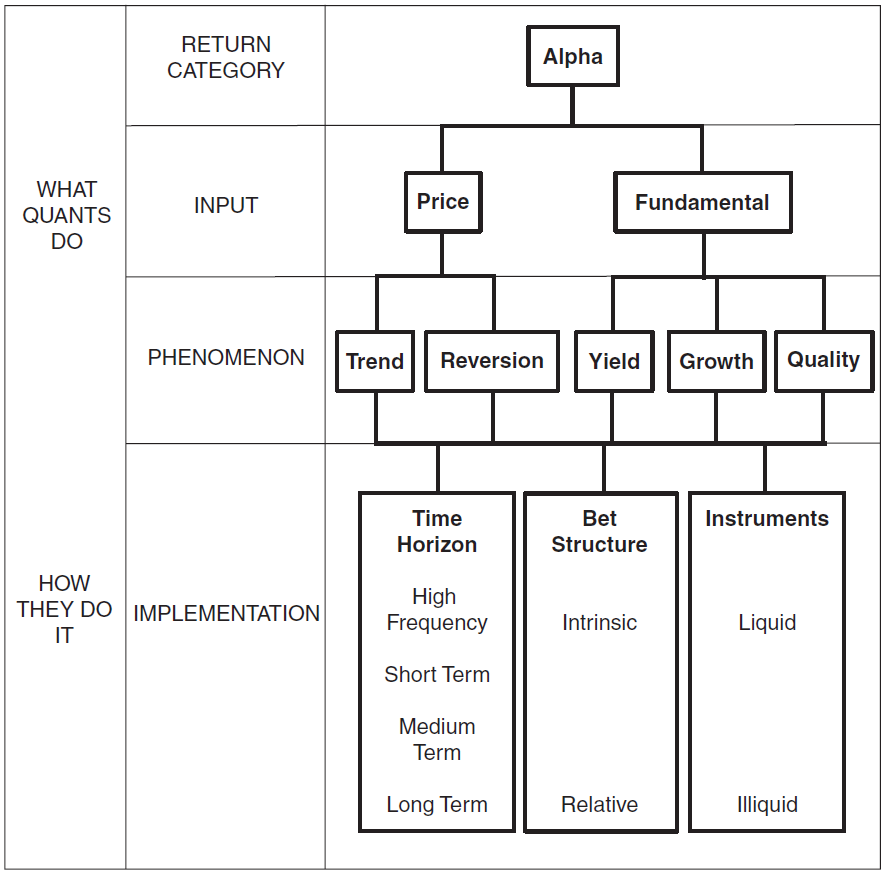
\includegraphics[width=.9\textwidth]{taxonomy.png}
					\caption{A taxonomy of theory-driven alpha models}
					\label{fig:taxonomy}
				\end{figure}


		\section{Blending alpha models}

			Each of the decisions a quant makes in defining a trading strategy is an important driver of its behavior. But there is another extremely important set of choices the quant must make in constructing a trading strategy. Specifically, the quant is not limited to choosing just one approach to a given alpha model. Instead, he is equally free to choose to employ \textit{multiple} types of alpha models. Even the method used to combine these alpha models is an arena rich with possibilities. The most sophisticated and successful quants tend to utilize several kinds of alpha strategies, including trend and reversion, and various kinds of fundamental approaches across a variety of time horizons, trade structures, instruments, and geographies. Such quants benefit from alpha diversification in exactly the same way that diversification is helpful in so many other aspects of financial life.

			The three most common quant approaches to blending forecasts are via \textit{linear models}, \textit{nonlinear models}, and \textit{machine learning models}. There is also a significant fourth school of thought that believes that alpha models should not be combined at all. Instead, several portfolios are constructed, each based on the output from a given alpha model. 

			Each of these four approaches to signal mixing has its disciples, and the best way to blend alphas depends on the model. In general, as in the case of an alpha model, the purpose of a method of mixing alpha models is to find the combination of them that best predicts the future. All other things being equal, it is very likely that any reasonably intelligent combination of alphas will do a better job together than any one of them could do individually over time. 

			Linear models are by far the most common way in which quants combine alpha factors to construct a composite forecast. A linear model is a reasonable facsimile for one of the more common ways that humans normally think about cause-and-effect relationships. In linear models, the inclusion of one factor is independent of the inclusion of other factors, and each factor is expected to be additive, independently of the other factors that might be included or excluded.

			The first step in using a linear model in this way is to assign a weight to each alpha factor. This is typically done using a technique known as \textit{multiple regression}, which is aimed at finding the combination of alpha factors that explains the maximum amount of the historical behavior of the instruments being traded. The presumption is that, if a model reasonably explains the past, it has a reasonable chance of explaining the future well enough to make a profit. These weights are then applied to the outputs of their respective alpha factors, which are usually a forecast or score of some kind. The weighted sum of these multiple forecasts gives us a combined forecast. Or, to be more specific, by summing the products of the weights of each factor and the outputs of each factor, we arrive at a composite forecast or score. This composite can then be used to help determine the target portfolio.

			A special case of linear models is the equal-weighted model. Though not highly quantitative, equal-weighting methods abound among quant traders. The general idea behind equal weighting is that the trader has no confidence in his ability to define more accurate weights and therefore decides to give all the alpha factors equal importance. A variant of this approach gives each factor an ``equal risk'' weighting, which incorporates the concept that giving a dollar to a highly risky strategy is not the same as giving a dollar to a less risky strategy.

			There are many forms of nonlinear models that can be used to combine alpha factors with each other. In contrast to linear models, nonlinear models are based on the premise that the relationship between the variables used to make forecasts either is not independent (i.e., each variable is not expected to add value independently of the others), or else the relationship changes over time. As such, the two main types of nonlinear models are conditional models and rotation models. Conditional models base the weight of one alpha factor on the reading of another factor. Using the same two factors as earlier, a conditional model might indicate that E/P yields should drive forecasts, but only when the price trends are in agreement with the E/P yields. In other words, the highest-yielding stocks would be candidates to be bought only if the price trends of these stocks were also positive. The lowest-yielding stocks would be candidates to be sold short, but only if the price trends of these stocks were also negative. When the agreement condition is met, the yield factor entirely drives the forecast. But if the price trend doesn't confirm the E/P yield signal, the yield signal is ignored entirely.

			The second nonlinear way to blend alphas uses a rotation approach. Rather than following trends in markets themselves, this type of model follows trends in the performance of the alpha models. These are similar to linear models except that the weights of factors fluctuate over time based on updated calculations of the various signals' weights. As time passes, the more recent data are used to determine weighting schemes in the hope that the model's weights are more relevant to current market conditions. This method usually results in giving higher weights to the factors that have performed better recently. As such, this is a form of trend following in the timing of alpha factors.

			Machine learning models are also sometimes used by quants to determine the optimal weights of various alpha factors. As in the case of determining optimal parameters, machine learning techniques applied to the mixing of alpha factors are both more common and more successful than machine learning approaches used to forecast markets themselves. These techniques algorithmically determine the mix of alpha factors that best explains the past, with the presumption that a good mix in the past is likely to be a good mix in the future. As in the case of rotational models, many machine learning approaches to mixing alpha factors periodically update the optimal weights based on the ever-changing and ever-growing set of data available. Unlike the example of using machine learning for the generation of actual alpha signals, applying machine learning to determine the weights of various alpha forecasts is more common and significantly more successful. Nevertheless, machine learning remains less widely used than the other techniques for blending alphas described here, and only a relatively small proportion of the universe of quant traders employ these methods.

			It is worth noting that signal mixing shares some similarities with portfolio construction. Both are questions of sizing and combining, after all. However, they are mostly distinct and separate processes. Signal-mixing models size multiple alpha signals to arrive at one composite forecast per security, which is then used in portfolio construction. Portfolio construction models take multiple kinds of signals as inputs, including alpha signals, risk models and transaction cost models, and attempt to size individual positions correctly, given these inputs.


\end{document}